\documentclass{beamer}

\mode<presentation>
{
  \usetheme{Warsaw}
  \useoutertheme{infolines}
  \usecolortheme{spruce}
  % or ...

  \setbeamercovered{transparent}
  % or whatever (possibly just delete it)
}

\usepackage{hyperref}
\usepackage{multicol}
\usepackage{graphicx}
\usepackage{verbatim}
\usepackage{amsmath}
\usepackage{listings}

\lstloadlanguages{C++}
\lstnewenvironment{code}
	{%\lstset{	numbers=none, frame=lines, basicstyle=\small\ttfamily, }%
	 \csname lst@SetFirstLabel\endcsname}
	{\csname lst@SaveFirstLabel\endcsname}
\lstset{% general command to set parameter(s)
	language=C++, basicstyle=\footnotesize\sffamily, keywordstyle=\slshape,
	emph=[1]{tipo,usa}, emphstyle={[1]\sffamily\bfseries},
	morekeywords={tint,forn,forsn},
	basewidth={0.47em,0.40em},
	columns=fixed, fontadjust, resetmargins, xrightmargin=5pt, xleftmargin=15pt,
	flexiblecolumns=false, tabsize=2, breaklines,	breakatwhitespace=false, extendedchars=true,
	numbers=left, numberstyle=\tiny, stepnumber=1, numbersep=9pt,
	frame=l, framesep=3pt,
}

\usepackage[spanish]{babel}
% or whatever

\usepackage[utf8]{inputenc}
% or whatever

\usepackage{times}
\usepackage[T1]{fontenc}
% Or whatever. Note that the encoding and the font should match. If T1
% does not look nice, try deleting the line with the fontenc.


\title[DP Avanzada] % (optional, use only with long paper titles)
{Temas Avanzados de Programación Dinámica}

\author[Agustín Gutiérrez] % (optional, use only with lots of authors)
{~Agustín Santiago Gutiérrez}
% - Give the names in the same order as the appear in the paper.
% - Use the \inst{?} command only if the authors have different
%   affiliation.
\institute[UBA] % (optional, but mostly needed)
{
  Facultad de Ciencias Exactas y Naturales\\
  Universidad de Buenos Aires
}
\date[TC 2017] % (optional, should be abbreviation of conference name)
{Training Camp Argentina 2017}

% Acá se puede insertar el logo de la UBA
% \pgfdeclareimage[height=0.5cm]{university-logo}{university-logo-filename}
% \logo{\pgfuseimage{university-logo}}



% Delete this, if you do not want the table of contents to pop up at
% the beginning of each subsection:
\AtBeginSubsection[]
{
  \begin{frame}{Contenidos}
  \footnotesize
    \tableofcontents[currentsection, currentsubsection]
  \end{frame}
}

% If you wish to uncover everything in a step-wise fashion, uncomment
% the following command: 

%\beamerdefaultoverlayspecification{<+->}


\begin{document}

\begin{frame}
  \titlepage
\end{frame}

\begin{frame}{Contenidos}
  \tableofcontents
  % You might wish to add the option [pausesections]
\end{frame}



\section{Repaso de Programación Dinámica}

\subsection{Dos visiones}

\begin{frame}{Visión tradicional}
	\begin{itemize}
		\item Programación Dinámica y Divide and Conquer son dos técnicas basadas en recursión
		\item En ambas queremos calcular algún(os) valor(es) de $f$, una función recursiva
		\item En divide and conquer, los subproblemas son completamente independientes entre sí, de modo que podemos implementar la recursión directa y resolver
		\item Se suele explicar programación dinámica, como ``Divide and Conquer, con memoria para reutilizar subproblemas repetidos''
	\end{itemize}
\end{frame}

\begin{frame}{Visión constructiva}
	\begin{itemize}
		\item Mi forma favorita de pensar programación dinámica
		\item Dado el problema que queremos encarar, imaginamos un ``proceso de construir una solución''
		\item El proceso parte de un \textbf{estado} inicial (eventualmente varios)
		\item Existen \textbf{transiciones} posibles, a través de las cuáles podemos pasar de un estado a otro
		\item El grafo de estados y transiciones define un DAG (si hay ciclos, no se puede aplicar DP)
		\item El estado \textbf{captura toda la información} que necesitamos \textbf{para seguir construyendo la solución} desde ese punto
	\end{itemize}
\end{frame}

\begin{frame}{Visión constructiva (cont)}
	\begin{itemize}
		\item El proceso de construcción de la solución consiste en recorrer un camino por los estados, hasta llegar a algún ``estado solución'' (casos base)
		\item Nuestro plan es calcular alguna ``cosa'' sobre las soluciones que se pueden construir desde cada estado
		\item Cosas típicas:
			\begin{itemize}
				 \item Cantidad de soluciones (cantidad de caminos)
				 \item Solución óptima (``mejor'' camino)
				 \item Solución lexicográficamente más chica
				 \item Conjunto de ``valores'' que puede tomar una solución (por ejemplo, conjunto de ``estados solución'' alcanzables desde cada estado)
			\end{itemize}
	\end{itemize}
\end{frame}


\begin{frame}{Ejemplos}
	\begin{itemize}
		\item Dominós en un tablero de $2 \times n$
		\item Cruzar la matriz
		\item Problema de la mochila
		\item ``Camino en DAG'' (mínimo, cantidad, etc). Con la visión constructiva, todo problema de DP es caso particular de este (como todos los anteriores)
	\end{itemize}
\end{frame}

\begin{frame}{Cómo se implementa con DP}
	\begin{itemize}
		\item Vamos a calcular con DP: $f(e) = \mbox{valor de la cosa que queremos calcular en el estado $e$}$
		\item Principio de optimalidad: Se podrá aplicar DP al problema, cuando para los estados elegidos se pueda calcular $f(e)$, a partir de los
		     $f(e_s)$ para todos los sucesores $e_s$ de $e$.
		\item A lo anterior nos referíamos cuando decíamos que el estado captura la información \textbf{necesaria}:
		   \begin{itemize}
			  \item Siempre podemos elegir un estado que haga válido el principio del óptimo. El trivial es tomar \textbf{todo el camino} recorrido como estado
			  \item La gran ganancia de programación dinámica surge de olvidar casi todos los detalles sobre el camino exacto utilizado, quedándose solamente con lo importante para poder completar la solución
			  \item Por ejemplo para mochila, no podemos sacar del estado la capacidad restante, o no sabremos si un objeto entra o no
		   \end{itemize}
	\end{itemize}
\end{frame}


\begin{frame}{Visión constructiva: Ventajas}
	\begin{itemize}
		\item Al reconstruir el camino, la reconstrucción lo recorre \textbf{en el orden del proceso de construcción de la solución} (``al derecho'').
		\item Por la propiedad anterior, es relativamente simple modificarlo para encontrar:
			\begin{itemize}
				\item La solución lexicográficamente más chica
				\item La solución lexicográficamente más grande
				\item Más en general, la $i$-ésima solución en orden lexicográfico (¡Notar que depende del orden! La visión constructiva ayuda a razonar en el orden en que queremos, \textbf{de entrada})
			\end{itemize}
		\item En mi experiencia personal subjetiva, esta forma de razonar me ayuda mucho a encontrar algoritmos de DP para problemas más difíciles.
		   \begin{itemize}
			\item Evidencia anecdótica: Cuando expliqué esta forma en una charla de DP en el TC UBA 2014, un equipo Cordobés me dijo que le encantó y que ``al fin entendimos lo que nuestro coach nos decía todo el tiempo: '¡Busquen el estado! ¡Busquen el estado!' ''
		   \end{itemize}
	\end{itemize}
\end{frame}

\subsection{Cosas calculables con visión constructiva}

\begin{frame}{Planteo}
	\begin{itemize}
		\item En todos los ejemplos que siguen, primero queremos plantear el proceso de crear una solución, como vimos
		\item Queremos plantearlo de forma que ``cada camino hasta un estado final'' lleve a una solución al problema
	\end{itemize}
\end{frame}

\begin{frame}{Conteo de soluciones}
	\begin{itemize}
		\item Contar cuántas soluciones hay, es contar caminos
		\item Usaremos la recursión $f(e) = \sum_{e_s}{f(e_s)}$, con $f(e) = 1$ para los estados finales
	\end{itemize}
\end{frame}

\begin{frame}{Solución lexicográficamente más chica}
	\begin{itemize}
		\item Suponemos que algunas soluciones ``funcionan'', y otras no. Queremos la lexicográficamente más chica que funciona
		\item Calculamos $f(e) = \mbox{desde $e$ se puede llegar a una solución que funciona}$
		\item Al reconstruir el camino, elegimos siempre el sucesor más chico que funciona
		\item Es muy común combinar esto con camino mínimo (solución óptima lexicográficamente más chica)
	\end{itemize}
\end{frame}

\begin{frame}{Solución $i$-ésima en orden lexicográfico}
	\begin{itemize}
		\item Suponemos que $i$ indexa desde $0$ (la solución $0$ es la que vimos antes, la lexicográficamente menor)
		\item En lugar de calcular solo si hay solución que funciona como en la anterior, las contamos sumando como ya vimos
		\item $f(e) = \mbox{Cantidad de soluciones que funcionan desde e}$
		\item Al reconstruir el camino, si buscamos la $i$-ésima y la primera opción tiene $T > i$ soluciones, nos movemos a esa opción
		\item Sino, le restamos $T$ a $i$, y verificamos lo mismo para la segunda opción.
		\item Seguimos así hasta mandarnos por una opción. Si ninguna funcionó, $i$ es demasiado grande y por lo tanto no hay $i$-ésima
		\item Cuando llegamos a un estado final con $i=0$, el camino que recorrimos describe la $i$-ésima solución
	\end{itemize}
\end{frame}

\section{Dinámicas con subconjuntos}

\subsection{Idea}

\begin{frame}{Idea}
\begin{itemize}
    \item El estado contiene un \textbf{subconjunto} $S \subseteq T$ de algún conjunto $T$ relevante al problema
    \item Implementación: número de $0$ a $2^n-1$ (máscara de bits: \texttt{0} a \texttt{(1<<n)-1})
       \begin{itemize}
		   \item $\cup$ es el \texttt{|}
		   \item $\cap$ es el \texttt{\&}
		   \item $\{ i \}$ es \texttt{1<<i}
		   \item $T$ es \texttt{(1<<n)-1}
		   \item $\emptyset$ es \texttt{0}
		   \item $S^c$ es \texttt{T\&(\textasciitilde S)} o \texttt{T-S}
		   \item $A - B = A \cap B^c$ es \texttt{A\&(\textasciitilde B)} o \texttt{A\&(T-S)}
       \end{itemize}
    \item Notar que el estado podría tener más cosas, o más de un subconjunto
\end{itemize}
\end{frame}

\subsection{Ejemplos}

\begin{frame}{Ejemplos}
    \begin{itemize}
		\item Matching perfecto de costo mínimo en grafo completo: $O(N2^N)$
		\pause
		\invisible<1>{
		\item Minimum set cover: $O(M2^N)$}
		\pause
		\invisible<1-2>{
		\item {\vfill TSP: $O(N^2 2^N)$ \vfill}		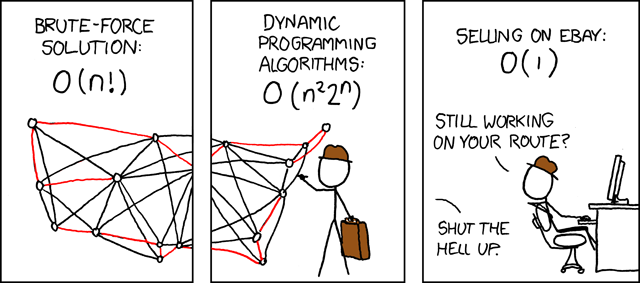
\includegraphics[scale = 0.3]{xkcd.png}
		\item Todas son \textbf{muchísimo} más eficientes que el backtracking directo}
    \end{itemize}
\end{frame}

\section{Dinámicas con frente}

\subsection{Idea}

\begin{frame}{Idea}
    \begin{itemize}
		\item Tenemos que considerar formas de ``llenar'' un tablero.
		\item Como siempre en programación dinámica, queremos ``olvidar lo más posible''
		\item Al ir llenando el tablero, suele alcanzar con saber únicamente la situación en el \textbf{frente} por dónde vamos llenando.
		\item Por ejemplo si queremos llenar un tablero con 0 y 1 pero sin que haya dos 1 pegados:
    \end{itemize}
    $$\begin{array}{cccc}
		? & ? & ? & ? \\
		? & ? & ? & ? \\
		? & ? & ? & ? \\
		? & ? & ? & ? \\
    \end{array}$$
\end{frame}

\begin{frame}{Idea}
    \begin{itemize}
		\item Tenemos que considerar formas de ``llenar'' un tablero.
		\item Como siempre en programación dinámica, queremos ``olvidar lo más posible''
		\item Al ir llenando el tablero, suele alcanzar con saber únicamente la situación en el \textbf{frente} por dónde vamos llenando.
		\item Por ejemplo si queremos llenar un tablero con 0 y 1 pero sin que haya dos 1 pegados:
    \end{itemize}
    $$\begin{array}{cccc}
		\color{red}0 & ? & ? & ? \\
		? & ? & ? & ? \\
		? & ? & ? & ? \\
		? & ? & ? & ? \\
    \end{array}$$
\end{frame}

\begin{frame}{Idea}
    \begin{itemize}
		\item Tenemos que considerar formas de ``llenar'' un tablero.
		\item Como siempre en programación dinámica, queremos ``olvidar lo más posible''
		\item Al ir llenando el tablero, suele alcanzar con saber únicamente la situación en el \textbf{frente} por dónde vamos llenando.
		\item Por ejemplo si queremos llenar un tablero con 0 y 1 pero sin que haya dos 1 pegados:
    \end{itemize}
    $$\begin{array}{cccc}
		\color{red}0 & ? & ? & ? \\
		\color{red}1 & ? & ? & ? \\
		? & ? & ? & ? \\
		? & ? & ? & ? \\
    \end{array}$$
\end{frame}


\begin{frame}{Idea}
    \begin{itemize}
		\item Tenemos que considerar formas de ``llenar'' un tablero.
		\item Como siempre en programación dinámica, queremos ``olvidar lo más posible''
		\item Al ir llenando el tablero, suele alcanzar con saber únicamente la situación en el \textbf{frente} por dónde vamos llenando.
		\item Por ejemplo si queremos llenar un tablero con 0 y 1 pero sin que haya dos 1 pegados:
    \end{itemize}
    $$\begin{array}{cccc}
		\color{red}0 & ? & ? & ? \\
		\color{red}1 & ? & ? & ? \\
		\color{red}1 & ? & ? & ? \\
		? & ? & ? & ? \\
    \end{array}$$
\end{frame}

\begin{frame}{Idea}
    \begin{itemize}
		\item Tenemos que considerar formas de ``llenar'' un tablero.
		\item Como siempre en programación dinámica, queremos ``olvidar lo más posible''
		\item Al ir llenando el tablero, suele alcanzar con saber únicamente la situación en el \textbf{frente} por dónde vamos llenando.
		\item Por ejemplo si queremos llenar un tablero con 0 y 1 pero sin que haya dos 1 pegados:
    \end{itemize}
    $$\begin{array}{cccc}
		\color{red}0 & ? & ? & ? \\
		\color{red}1 & ? & ? & ? \\
		\color{red}1 & ? & ? & ? \\
		\color{red}0 & ? & ? & ? \\
    \end{array}$$
\end{frame}

\begin{frame}{Idea}
    \begin{itemize}
		\item Tenemos que considerar formas de ``llenar'' un tablero.
		\item Como siempre en programación dinámica, queremos ``olvidar lo más posible''
		\item Al ir llenando el tablero, suele alcanzar con saber únicamente la situación en el \textbf{frente} por dónde vamos llenando.
		\item Por ejemplo si queremos llenar un tablero con 0 y 1 pero sin que haya dos 1 pegados:
    \end{itemize}
    $$\begin{array}{cccc}
		0 & \color{red}1 & ? & ? \\
		\color{red}1 & ? & ? & ? \\
		\color{red}1 & ? & ? & ? \\
		\color{red}0 & ? & ? & ? \\
    \end{array}$$
\end{frame}

\begin{frame}{Idea}
    \begin{itemize}
		\item Tenemos que considerar formas de ``llenar'' un tablero.
		\item Como siempre en programación dinámica, queremos ``olvidar lo más posible''
		\item Al ir llenando el tablero, suele alcanzar con saber únicamente la situación en el \textbf{frente} por dónde vamos llenando.
		\item Por ejemplo si queremos llenar un tablero con 0 y 1 pero sin que haya dos 1 pegados:
    \end{itemize}
    $$\begin{array}{cccc}
		0 & \color{red}1 & ? & ? \\
		1 & \color{red}0 & ? & ? \\
		\color{red}1 & ? & ? & ? \\
		\color{red}0 & ? & ? & ? \\
    \end{array}$$
\end{frame}

\begin{frame}{Idea}
    \begin{itemize}
		\item Tenemos que considerar formas de ``llenar'' un tablero.
		\item Como siempre en programación dinámica, queremos ``olvidar lo más posible''
		\item Al ir llenando el tablero, suele alcanzar con saber únicamente la situación en el \textbf{frente} por dónde vamos llenando.
		\item Por ejemplo si queremos llenar un tablero con 0 y 1 pero sin que haya dos 1 pegados:
    \end{itemize}
    $$\begin{array}{cccc}
		0 & \color{red}1 & ? & ? \\
		1 & \color{red}0 & ? & ? \\
		1 & \color{red}0 & ? & ? \\
		\color{red}0 & ? & ? & ? \\
    \end{array}$$
\end{frame}

\begin{frame}{Idea}
    \begin{itemize}
		\item Tenemos que considerar formas de ``llenar'' un tablero.
		\item Como siempre en programación dinámica, queremos ``olvidar lo más posible''
		\item Al ir llenando el tablero, suele alcanzar con saber únicamente la situación en el \textbf{frente} por dónde vamos llenando.
		\item Por ejemplo si queremos llenar un tablero con 0 y 1 pero sin que haya dos 1 pegados:
    \end{itemize}
    $$\begin{array}{cccc}
		0 & \color{red}1 & ? & ? \\
		1 & \color{red}0 & ? & ? \\
		1 & \color{red}0 & ? & ? \\
		0 & \color{red}1 & ? & ? \\
    \end{array}$$
\end{frame}

\begin{frame}{Idea}
    \begin{itemize}
		\item Tenemos que considerar formas de ``llenar'' un tablero.
		\item Como siempre en programación dinámica, queremos ``olvidar lo más posible''
		\item Al ir llenando el tablero, suele alcanzar con saber únicamente la situación en el \textbf{frente} por dónde vamos llenando.
		\item Por ejemplo si queremos llenar un tablero con 0 y 1 pero sin que haya dos 1 pegados:
    \end{itemize}
    $$\begin{array}{cccc}
		0 & 1 & \color{red}0 & ? \\
		1 & \color{red}0 & ? & ? \\
		1 & \color{red}0 & ? & ? \\
		0 & \color{red}1 & ? & ? \\
    \end{array}$$
\end{frame}

\begin{frame}{Idea}
    \begin{itemize}
		\item Tenemos que considerar formas de ``llenar'' un tablero.
		\item Como siempre en programación dinámica, queremos ``olvidar lo más posible''
		\item Al ir llenando el tablero, suele alcanzar con saber únicamente la situación en el \textbf{frente} por dónde vamos llenando.
		\item Por ejemplo si queremos llenar un tablero con 0 y 1 pero sin que haya dos 1 pegados:
    \end{itemize}
    $$\begin{array}{cccc}
		0 & 1 & \color{red}0 & ? \\
		1 & 0 & \color{red}0 & ? \\
		1 & \color{red}0 & ? & ? \\
		0 & \color{red}1 & ? & ? \\
    \end{array}$$
\end{frame}

\begin{frame}{Estado}
    \begin{itemize}
		\item El estado tendrá la posición $(x,y)$ actual en el tablero.
		\item Además, para un tablero de $N \times M$, guardará $N$ valores (o a veces $N+1$) con el frente.
		\item Si los valores son binarios como en el ejemplo hay $O(NM2^N)$ estados, pero en cambio hay $2^{NM}$ tableros.
	\end{itemize}
\end{frame}


\subsection{Ejemplos}

\begin{frame}{Ejemplos}
    \begin{itemize}
		\item Cantidad de maneras de cubrir con dominós, un tablero con agujeros en posiciones dadas
		\pause
		\invisible<1>{
		\item Cantidad de maneras de cubrir con ``tuberías'' cerradas (ciclos), un tablero con agujeros en posiciones dadas \\
		{\hfill 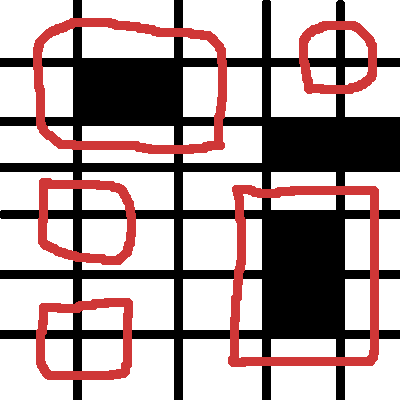
\includegraphics[scale = 0.25]{tuberias.png} \hfill}
		}
		\pause
		\invisible<1-2>{
		\item El frente anterior tiene $O(2^N)$ valores posibles. ¿Y si quisiéramos saber la mínima cantidad de ciclos necesarios?
		}
		\pause
		\invisible<1-3>{
		\item Se puede con un frente con $O(3^N)$ valores posibles.
		}
    \end{itemize}
\end{frame}

\section{Técnicas de optimización de DP}

\subsection{Optimización de Knuth}

\begin{frame}{Ejemplo motivador}
    \begin{itemize}
		\item Dados $n$ valores enteros distintos $v_i$, junto a sus frecuencias $f_i$, dar un árbol binario de búsqueda óptimo para los valores.
		\pause
		\invisible<1>{
			\item $dp(i,j) = \mbox{min}_{k=i}^{j-1}{\ dp(i,k) + dp(k+1,j) + sum_f(i,j)}$
			\item Complejidad: $O(n^3)$
			\item ¿Se podrá mejorar?
		}
    \end{itemize}
\end{frame}

\begin{frame}{Contexto}
    \begin{itemize}
		\item ¡Sí! Con la optimización de Knuth
		\item Dado un algoritmo de dp en rangos cualquiera, es decir \\ $dp(i,j)$ con $0 \leq i \leq j \leq N$
		\item Si su recursión tiene la forma $dp(i,j) = \mbox{min}_{k=i}^{j-1}{\ g(i,k,j)}$ para cierta $g$ que solo usa los rangos $dp(a,b)$ contenidos en $(i,j)$
		\item Podemos definir $K(i,j)$ como el menor $k$ en donde se alcanza el mínimo de la expresión para $dp(i,j)$
    \end{itemize}
\end{frame}

\begin{frame}{Condición de Knuth}
    \begin{itemize}
		\item $K(i,j-1) \leq K(i,j) \leq K(i+1, j)$
		\item En criollo:
		  \begin{itemize}
			\item Si agregamos un elemento por \textbf{izquierda}, \\ el $K$ se mueve \textbf{a la izquierda}
			\item Si agregamos un elemento por \textbf{derecha}, \\ el $K$ se mueve \textbf{a la derecha}
		  \end{itemize}
		\item Llamamos a la anterior la \textit{Condición de Knuth}
		\item Suele ser mucho más difícil demostrar que se cumple, que convencerse o intuir que así será
    \end{itemize}
\end{frame}

\begin{frame}{Optimización de Knuth}
    \begin{itemize}
		\item Como vale la condición de Knuth, es muy simple cambiar en el código la recursión usando las cotas para iterar menos:
		\item $dp(i,j) = \mbox{min}_{k=K(i,j-1)}^{K(i+1,j)}{\ g(i,k,j)}$
		\item Los $K$ los podemos ir calculando en el mismo algoritmo junto a los valores $dp$.
		\item Las cotas sirven para iterar menos... ¿Pero estamos mejorando la complejidad asintótica?
		\pause
		\invisible<1>{
			\item Teorema: Con este sencillísimo cambio al código básico, el algoritmo es $O(N^2)$
			\item Demostración: La sumatoria de los costos es telescópica en 2D
			\item Si evaluar $g$ no es $O(1)$, el costo son $O(N^2)$ evaluaciones de $g$
		}
    \end{itemize}
\end{frame}

\begin{frame}{Ejercicio}
    \begin{itemize}
		\item Ejercicio: Verificar que la condición de Knuth aplica en la recursión que vimos antes 
		\item Intuitivamente tiene muchísimo sentido, ¡pero demostrarlo es mucho más difícil que programarlo!
    \end{itemize}
\end{frame}


\subsection{Optimización de Divide and Conquer}

\begin{frame}{Ejemplo motivador}
    \begin{itemize}
		\item Dados $n$ valores $x_i$ enteros positivos, el costo de un intervalo $[i,j)$ es $\sum_{i \leq a<b<j}{x_a x_b} $. O sea, sumar los productos de a pares.
		\item Particionar el arreglo $[0,n)$ en $k$ intervalos, minimizando la suma de los $k$ costos.
		\pause
		\invisible<1>{
			\item $dp(n,k) = \mbox{min}_{i=0}^{n-1}{\ dp(i,k-1) + val(i,n)}$
			\item Complejidad: $O(n^2 k)$
			\item ¿Se podrá mejorar?
		}
    \end{itemize}
\end{frame}

\begin{frame}{Contexto}
    \begin{itemize}
		\item ¡Sí! Con la optimización de Divide and Conquer
		\item Dado un algoritmo de dp ``de particionar'' cualquiera, es decir \\ $dp(n,k)$ con $0 \leq n \leq N$ y $0 \leq k \leq K$
		\item Si su recursión tiene la forma $dp(n,k) = \mbox{min}_{i=0}^{n-1}{\ g(n,k,i)}$ para cierta $g$ que solo usa los $dp(j,k-1)$ 
		\item Podemos definir $I(n,k)$ como el menor $i$ en donde se alcanza el mínimo de la expresión para $dp(n,k)$
    \end{itemize}
\end{frame}

\begin{frame}{Condición de Divide and Conquer}
    \begin{itemize}
		\item $I(n,k) \leq I(n+1,k)$
		\item Para cada $k$, el $I$ es creciente en $n$.
		\item En criollo: si para $k$ fijo agrando el rango, el último punto de corte también (mejor dicho: no retrocede) 
		\item Llamamos a la anterior la \textit{Condición de Divide and Conquer}
		\item Igual que antes, suele ser mucho más difícil demostrar que se cumple, que convencerse o intuir que así será
    \end{itemize}
\end{frame}

\begin{frame}{Optimización de Divide and Conquer}
    \begin{itemize}
		\item Esta optimización no es tan simple de implementar como la de Knuth, pero la idea también es sencilla.
		\item Supongamos que para calcular todos los $dp(n,k)$ para $k$ fijo, calculamos primero el $dp(n',k)$:
			\begin{itemize}
				\item Para los $n > n'$, alcanza con probar el $i$ \textbf{desde} $I(n',k)$ \\
						Es decir, no más de $L_1 = n - I(n',k) + 1$ valores
				\item Para los $n < n'$, alcanza con probar el $i$ \textbf{hasta} $I(n',k)$ \\
				        Es decir, no más de $L_2 = I(n',k) + 1$ valores
			\end{itemize}
		\item Esto nos parte el rango $[0,N)$ que debíamos calcular en dos restantes: $[0,n')$ y $[n'+1,N)$.
		\item En la primera parte hay que probar hasta $L_1$ valores, y en la segunda hasta $L_2$ valores.
    \end{itemize}
\end{frame}

\begin{frame}{Si profundizamos...}
    \begin{itemize}
		\item Podemos seguir partiendo estos rangos en dos recursivamente
		\item En el paso $k$ tendremos $2^k$ rangos, cada uno con hasta $L_i$ opciones factibles para el $i$.
		\item Observación: En cada paso, los $L_i$ suman $O(N)$
		\item Por lo tanto, procesar cada paso es $O(N)$
		\item Partiendo siempre a la mitad, serán $O(\lg N)$ pasos y la complejidad es $O(N \lg N)$
		\item El algoritmo final resulta costar $O(KN\lg N)$ evaluaciones de $g$
    \end{itemize}
\end{frame}



\begin{frame}{Ejercicio}
    \begin{itemize}
		\item Ejercicio: Verificar que la condición de Divide and Conquer aplica en la recursión que vimos antes 
		\item Pasa lo mismo que antes: Es más fácil intuirlo que probarlo
    \end{itemize}
\end{frame}


\end{document}
